\documentclass[12pt,a4paper]{report}

\usepackage[utf8x]{inputenc}
\usepackage{amsmath}
\usepackage{amsfonts}
\usepackage{amssymb}
\usepackage{graphicx}
\usepackage{enumitem}
\usepackage{fontspec}
\usepackage{pgf}
\usepackage{tikz}
\usepackage{calrsfs}
\usepackage{ifthen}
\usepackage{algpseudocode}
%\usepackage[linesnumbered,lined,boxed,commentsnumbered]{algorithm2e}
\usetikzlibrary{graphs, shapes, snakes, graphdrawing}
\usegdlibrary{layered, force}

\begin{document}

\begin{titlepage}
	\centering
	{\scshape\LARGE Universidad Nacional Autónoma de México \par}
	\vspace{1cm}
	{\scshape\Large Computación Distribuida\par}
	\vspace{1.5cm}
	{\huge\bfseries Tarea 3\par}
	\vspace{.5cm}
	{\Large\itshape Edgar Quiroz Castañeda \par}
    \vspace{.5cm}
	{\Large\itshape Jerónimo Almeida Rodríguez \par}
	\vfill
	 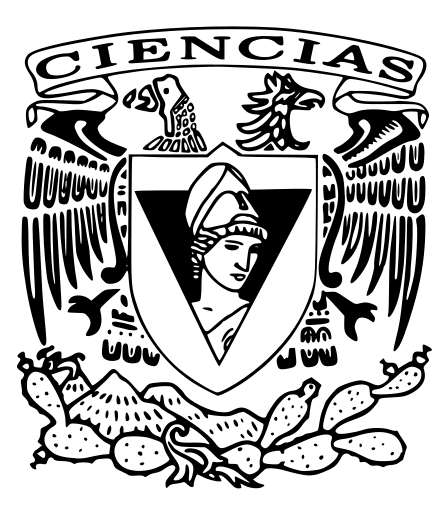
\includegraphics[width=0.5\textwidth]{escudo_f-ciencias.png}
	\vfill

% Bottom of the page
	{\large Jueves 30 de Agosto del 2018 \par}
\end{titlepage}

\pagebreak
\setlength{\voffset}{-0.75in}
\setlength{\headsep}{5pt}

%\newcommand{\ed}[2]{(#1) edge (#2)}
%\newcommand{\eee}[4]{\path [->,draw,thin] ($ (#1) !.5! (#2)$) -- ($ (#3) !.5! (#4) $);}

\newcommand{\is}[1]{V_{\{B, x, r\}}}

\begin{enumerate}
	%Ejercicio 1
	\item {
		Dados los procesos $A$ y $B$, diseña un algoritmo para el ataque coordinado
		proximado (aproximate agreement) en el que para llegar al acuerdo deben
		decidir	valores que estén a distancia a lo más $\frac{1}{2^k}$ y utilice menos
		rondas de comunicación que el algoritmo visto en clase.\\

		El algoritmo propuesto es el siguiente:\\

		\begin{algorithmic}[1]
			\Require $id \in \{A,B\},\ init \in \{0, 1\},\ k \in \mathbb{N}$
			\Ensure $v_A^k\ \& \ v_B^k$ tales que $|v_A^k\ - \ v_B^k|\ \leq\ \dfrac{1}
				{2^k}$
			\Function{\textbf{ Modelo:}$\{A\leftrightarrow B, A \rightarrow B, 
				A \leftarrow B\}$}{$init$}			
				\State $v\ \leftarrow init$
				\For{r = 0 \textbf{to} k + 1}{}
					\State $send(v)$
					\State $msg \leftarrow$ receive()
					\If{$msg \ne null$}
						\If{$msg = v$}
							\State break
						\Else	
							\State $v \leftarrow \dfrac{v + msg}{2}$
						\EndIf
					\EndIf
				\EndFor
				\State \Return$v$
			\EndFunction
		\end{algorithmic}
	}
	

	\textbf{Demostración:}\\
	S.P.G. proponemos a la variable $\is{B}$ dónde $V$ representa la
	invariante de ciclo y el vector $\{B, x, r\}$ en el subíndice representa el
	nombre del proceso, su	valor actual y el número de ronda actual
	respectivamente.\\\\
	Por el teorema visto con Karla en clase sabemos que en la ronda $r$ hay
	comunicación perfecta, entonces $\ v_A^k\  =\  v_B^k\ $ en la ronda $r + 1$.\\
	


	%Ejercicio 2
	\item {
		Dibuja la gráfica del protocolo que diseñaste para 2 rondas para $k = 2$.
		Para cada vértice indica el valor de salida y para cada arista indica el
		patrón de mensajes recibidos.\\\\

		\begin{tikzpicture}[scale = 2]
			\tikzstyle{every node} = [draw, shape = circle]
			\foreach \i/\s in {0/$A \longrightarrow B$, 2/$A\longleftarrow B$}{
				\node at (\i, 9) (Bu\i) [label = above : {1}] {$B$};
				\node at (\i + 1, 9) (Au\i) [label = above : {1}] {$A$};
				\ifthenelse{\i = 2}{\draw (Au0) -- node[above,draw=none]{$A\longleftrightarrow B$}++(Bu\i);}{}
				\draw (Au\i) --node[above, draw=none, label = above : {\s}]{\s}++ (Bu\i) ;
				\node at (\i, 0) (Al\i) [label = below : {0}] {$A$};
				\node at (\i + 1, 0) (Bl\i) [label = below : {0}] {$B$};
				\ifthenelse{\i = 2}{\draw (Bl0) -- node[below,draw=none]{$A\longleftrightarrow B$}++ (Al\i);}{}
				\draw (Al\i) --node[below, draw=none, label = below : {\s}]{\s}++ (Bl\i);
			}
			\foreach \i/\j/\k in {2/0/1, 4/2/2, 6/4/2, 8/6/3}{

				\node at (0, \i) (Ai\i) [label = left : {\k/4}] {$A$};
				\node at (0, \i - 1) (Bi\i) [label = left : {\k/4}] {$B$};

				\ifthenelse{\i = 4}{\draw (Ai\j) -- node[rectangle, left, draw=none, label = left : {$A \longleftarrow B$}]{$A \longrightarrow B$}++ (Bi\i);}{}
				\ifthenelse{\i = 6}{\draw (Ai\j) -- node[rectangle, left, draw=none, label = left : {$A \longleftrightarrow B$}]{$A \longleftrightarrow B$}++ (Bi\i);}{}
				\ifthenelse{\i = 8}{\draw (Ai\j) -- node[rectangle, left, draw=none, label = left : {$A \longrightarrow B$}]{$A \longleftarrow B$}++ (Bi\i);}{}

				\ifthenelse{\i = 2}{\draw (Ai\i) -- node[rectangle, left, draw=none, label = left : {$A \longleftrightarrow B$}]{$A \longrightarrow B$}++ (Bi\i);}{}
				\ifthenelse{\i = 4}{\draw (Ai\i) -- node[rectangle, left, draw=none, label = left : {$A \longleftarrow B$}]{$A \longleftrightarrow B$}++ (Bi\i);}{}
				\ifthenelse{\i = 6}{\draw (Ai\i) -- node[rectangle, left, draw=none, label = left : {$A \longrightarrow B$}]{$A \longleftrightarrow B$}++ (Bi\i);}{}
				\ifthenelse{\i = 8}{\draw (Ai\i) -- node[rectangle, left, draw=none, label = left : {$A \longleftrightarrow B$}]{$A \longleftarrow B$}++ (Bi\i);}{}
				%\draw (Ai\i) -- node[rectangle, left, draw=none, label = left : {\s}]{\s} (Bi\i);

				\node at (3, \i - 1) (Ad\i) [label = right : {\k/4}] {$A$};
				\node at (3, \i) (Bd\i) [label = right : {\k/4}] {$B$};

				\ifthenelse{\i = 4}{\draw (Bd\j) -- node[rectangle, right, draw=none, label = right : {$A \longrightarrow B$}]{$A \longleftarrow B$}++ (Ad\i);}{}
				\ifthenelse{\i = 6}{\draw (Bd\j) -- node[rectangle, right, draw=none, label = right : {$A \longleftrightarrow B$}]{$A \longleftrightarrow B$}++ (Ad\i);}{}
				\ifthenelse{\i = 8}{\draw (Bd\j) -- node[rectangle, right, draw=none, label = right : {$A \longleftarrow B$}]{$A \longrightarrow B$}++ (Ad\i);}{}

				\ifthenelse{\i = 2}{\draw (Ad\i) -- node[rectangle, right, draw=none, label = right : {$A \longleftrightarrow B$}]{$A \longleftarrow B$}++ (Bd\i);}{}
				\ifthenelse{\i = 4}{\draw (Ad\i) -- node[rectangle, right, draw=none, label = right : {$A \longrightarrow B$}]{$A \longleftrightarrow B$}++ (Bd\i);}{}
				\ifthenelse{\i = 6}{\draw (Ad\i) -- node[rectangle, right, draw=none, label = right : {$A \longleftarrow B$}]{$A \longleftrightarrow B$}++ (Bd\i);}{}
				\ifthenelse{\i = 8}{\draw (Ad\i) -- node[rectangle, right, draw=none, label = right : {$A \longleftrightarrow B$}]{$A \longrightarrow B$}++ (Bd\i);}{}
				%\draw (Ad\i) -- node[rectangle, right, draw=none, label = right : {\l}]{\l}++ (Bd\i);
			}
			\draw (Al0) -- node[rectangle, left, draw=none, label = left : {$A \longrightarrow B$}]{$A \longrightarrow B$}++ (Bi2);
			\draw (Bl2) -- node[rectangle, right, draw=none, label = right : {$A \longleftarrow B$}]{$A \longleftarrow B$}++(Ad2);
			\draw (Ai8) -- node[rectangle, left, draw=none, label = left : {$A \longleftarrow B$}]{$A \longleftarrow B$}++(Bu0);
			\draw (Bd8) -- node[rectangle, right, draw=none, label = right : {$A \longrightarrow B$}]{$A \longrightarrow B$}++ (Au2);
		\end{tikzpicture}

		En la gráfica, los números cercanos a los vértices son el estado final de
		procesos, y las flechas indican la secuencia de comunicación que hubo,
		siendo el primer paso el más cercano a la gráfica.\\
		Las partes laterales de la gráfica son exactamente iguales a los de la
		gráfica obtenida con el acuerdo aproximado visto en clase. Esto es porque
		es imposible llegar a un punto en el que ambos procesos tienen un mismo
		valor y alguno de ellos lo sabe en menos de dos rondas.
		Aunque de realizar más rondas se notaría este patrón de menos posibles casos
		en las regiones donde hay al menos una ronda de comunicación perfecta, y
		los casos dejaría de subdividirse cuando lleguen a dos rondas de comunicación
		perfecta.
		Pero ya en dos rondas, se nota como en la parte superior y inferior, que
		corresponden a cuando los procesos tienen entradas iguales, hay menos posibles
		casos.
		Esto sucede de dos maneras.
		Puede ser que en la primera ronda haya comunicación perfecta, por lo que
		ambos procesosse detienen sin realizar la segunda ronda.
		Esto corresponde a la arista central, que se puede ver sólo tiene una ronda
		de comunicación registrada.
		O puede ser que haya algún mensaje se pierda, por lo que un proceso se
		detendría pero el otro seguiría con la siguiete ronda. Entonces si hay algún
		error de comunicación, la única posibibilidad en la siguieteronda es que
		el proceso que no recibió mensaje lo envía. Por esto es que se reducen los
		casos.
	}


\end{enumerate}
\end{document}